\documentclass[10pt]{article}
\usepackage[letterpaper,text={6.5in,8.7in},centering]{geometry}
\usepackage{amssymb,amsmath,times,url,subfigure,graphicx,theorem,alltt,eepic,epic,color,tikz}
%\usepackage[pdftex,urlcolor=blue,pdfpagemode=none,pdfstartview=FitH]{hyperref}

%% url smaller font.
\makeatletter
\def\url@leostyle{%
  \@ifundefined{selectfont}{\def\UrlFont{\sf}}{\def\UrlFont{\small\ttfamily}}}
\makeatother
\urlstyle{leo}

%\usepackage[all,import]{xy}

\newcommand{\norm}[1]{\ensuremath{\left\| #1 \right\|}}
\newcommand{\abs}[1]{\ensuremath{\left| #1 \right|}}
\newcommand{\bracket}[1]{\ensuremath{\left[ #1 \right]}}
\newcommand{\braces}[1]{\ensuremath{\left\{ #1 \right\}}}
\newcommand{\parenth}[1]{\ensuremath{\left( #1 \right)}}
\newcommand{\ip}[1]{\ensuremath{\langle #1 \rangle}}
\newcommand{\refeqn}[1]{(\ref{eqn:#1})}
\newcommand{\reffig}[1]{Fig. \ref{fig:#1}}
\newcommand{\tr}[1]{\mbox{tr}\ensuremath{\negthickspace\bracket{#1}}}
\newcommand{\deriv}[2]{\ensuremath{\frac{\partial #1}{\partial #2}}}
\newcommand{\SO}{\ensuremath{\mathrm{SO(3)}}}
\newcommand{\T}{\ensuremath{\mathrm{T}}}
\newcommand{\so}{\ensuremath{\mathfrak{so}(3)}}
\newcommand{\SE}{\ensuremath{\mathrm{SE(3)}}}
\newcommand{\se}{\ensuremath{\mathfrak{se}(3)}}
\renewcommand{\Re}{\ensuremath{\mathbb{R}}}
\renewcommand{\S}{\ensuremath{\mathbb{S}}}
\newcommand{\aSE}[2]{\ensuremath{\begin{bmatrix}#1&#2\\0&1\end{bmatrix}}}
\newcommand{\ase}[2]{\ensuremath{\begin{bmatrix}#1&#2\\0&0\end{bmatrix}}}
\newcommand{\D}{\ensuremath{\mathbf{D}}}
\newcommand{\pair}[1]{\ensuremath{\left\langle #1 \right\rangle}}
\newcommand{\met}[1]{\ensuremath{\langle\!\langle #1 \rangle\!\rangle}}
\newcommand{\Ad}{\ensuremath{\mathrm{Ad}}}
\newcommand{\ad}{\ensuremath{\mathrm{ad}}}
\newcommand{\g}{\ensuremath{\mathfrak{g}}}

\renewcommand{\baselinestretch}{1.2}
\date{}

\renewcommand{\thesubsection}{\arabic{subsection}. }
\renewcommand{\thesubsubsection}{\arabic{subsection}.\arabic{subsubsection} }

\theoremstyle{plain}\theorembodyfont{\normalfont}
\newtheorem{prob}{Problem}[section]
%\renewcommand{\theprob}{\arabic{section}.\arabic{prob}}
\renewcommand{\theprob}{\arabic{prob}}

\newenvironment{subprob}%
{\renewcommand{\theenumi}{\alph{enumi}}\renewcommand{\labelenumi}{(\theenumi)}\begin{enumerate}}%
{\end{enumerate}}%

\newenvironment{matlab}
{\begin{alltt}\small\renewcommand{\baselinestretch}{1.2}\selectfont}%
{\end{alltt}}

\newcommand*\circled[1]{%
  \tikz[baseline=(C.base)]\node[draw,circle,inner sep=0.5pt](C) {#1};\!
}

\begin{document}

\pagestyle{empty}
\section*{MAE3145: Homework 5}
\vspace*{-0.4cm}
\noindent{Due date: December 7, 2016}%\\%\vspace*{0.5cm}

\begin{prob}
Consider a reentry vehicle at the point $A$ on a circular orbit around the Earth. We wish to design a reentry orbit such that the vehicle arrives at $B$ along a trajectory tangent to the surface of the Earth at $B$, i.e. the point $B$ is the periapsis of the reentry orbit. 

\definecolor{gray}{rgb}{0.1, 0.1, 0.1}
\centerline{
\setlength{\unitlength}{1.5em}\centering\small
\begin{picture}(10,10)(-5,-5)
{\filltype{shade}\put(0,0){\circle*{4}}}
\put(0,0){\vector(1,0){4.8}}
\put(0,0){\vector(0,1){4.8}}
\put(0,0){\circle{8}}
\put(-3.4641,-2){\circle*{0.15}}
\put(2,0){\circle*{0.15}}
\put(-3.9,-2.5){$A$}
\put(2.1,-0.5){$B$}
\put(5.0,-0.4){$\hat x$}
\put(0.3,4.5){$\hat y$}
%\linethickness{8pt}
\put(-0.5,-1.0){Earth}
\end{picture}}
\vspace*{-0.3cm}
%
\noindent The initial circular orbit is referred to as Orbit 1, and the reentry orbit is referred to as Orbit 2. We do not consider the atmospheric drag effects. Assume that
\begin{gather*}
R_1 = 7000\,\mathrm{km},\quad R_E=6378\,\mathrm{km},\quad \mu=398600\,\mathrm{km^3/s^2},\quad \theta_A=210^\circ.
\end{gather*}
Recall that the velocity vector of a mass located at $\theta$ on an orbit with $h,e$ is given by
\begin{align*}
\vec v = \frac{\mu}{h} [-\sin\theta \hat x + (e+\cos\theta)\hat y].
\end{align*}

\begin{subprob}
\item Find the velocity vector $\vec v_{A_1}$ of the reentry vehicle at the point $A$ on Orbit 1.
\item Find the eccentricity $e_2$ and the specific angular momentum $h_2$ of Orbit 2.
\item Find the velocity vector $\vec v_{A_2}$ of the reentry vehicle at the point $A$ on Orbit 2.
\item Find the required velocity change $\vec v_A$ at the point $A$.
\item Find the resulting velocity $\vec v_{B_2}$ of the reentry vehicle at the surface of the Earth.
\end{subprob}
\end{prob}

\begin{prob}
We solve Exercise 6.21 of the textbook. Two spacecraft are on the same elliptic orbit with $r_p=8000\,\mathrm{km}$, $r_a=13000\,\mathrm{km}$. Currently, Spacecraft 1 is at the point $P$ ($\theta_P=0$), and Spacecraft 2 is at the point $C$ ($\theta_C=30^\circ$). We will find the velocity change for Spacecraft 1 to intercept and rendezvous with Spacecraft 2 at the point $D$ ($\theta_D=90^\circ$).

\vspace*{0.2cm}
\centerline{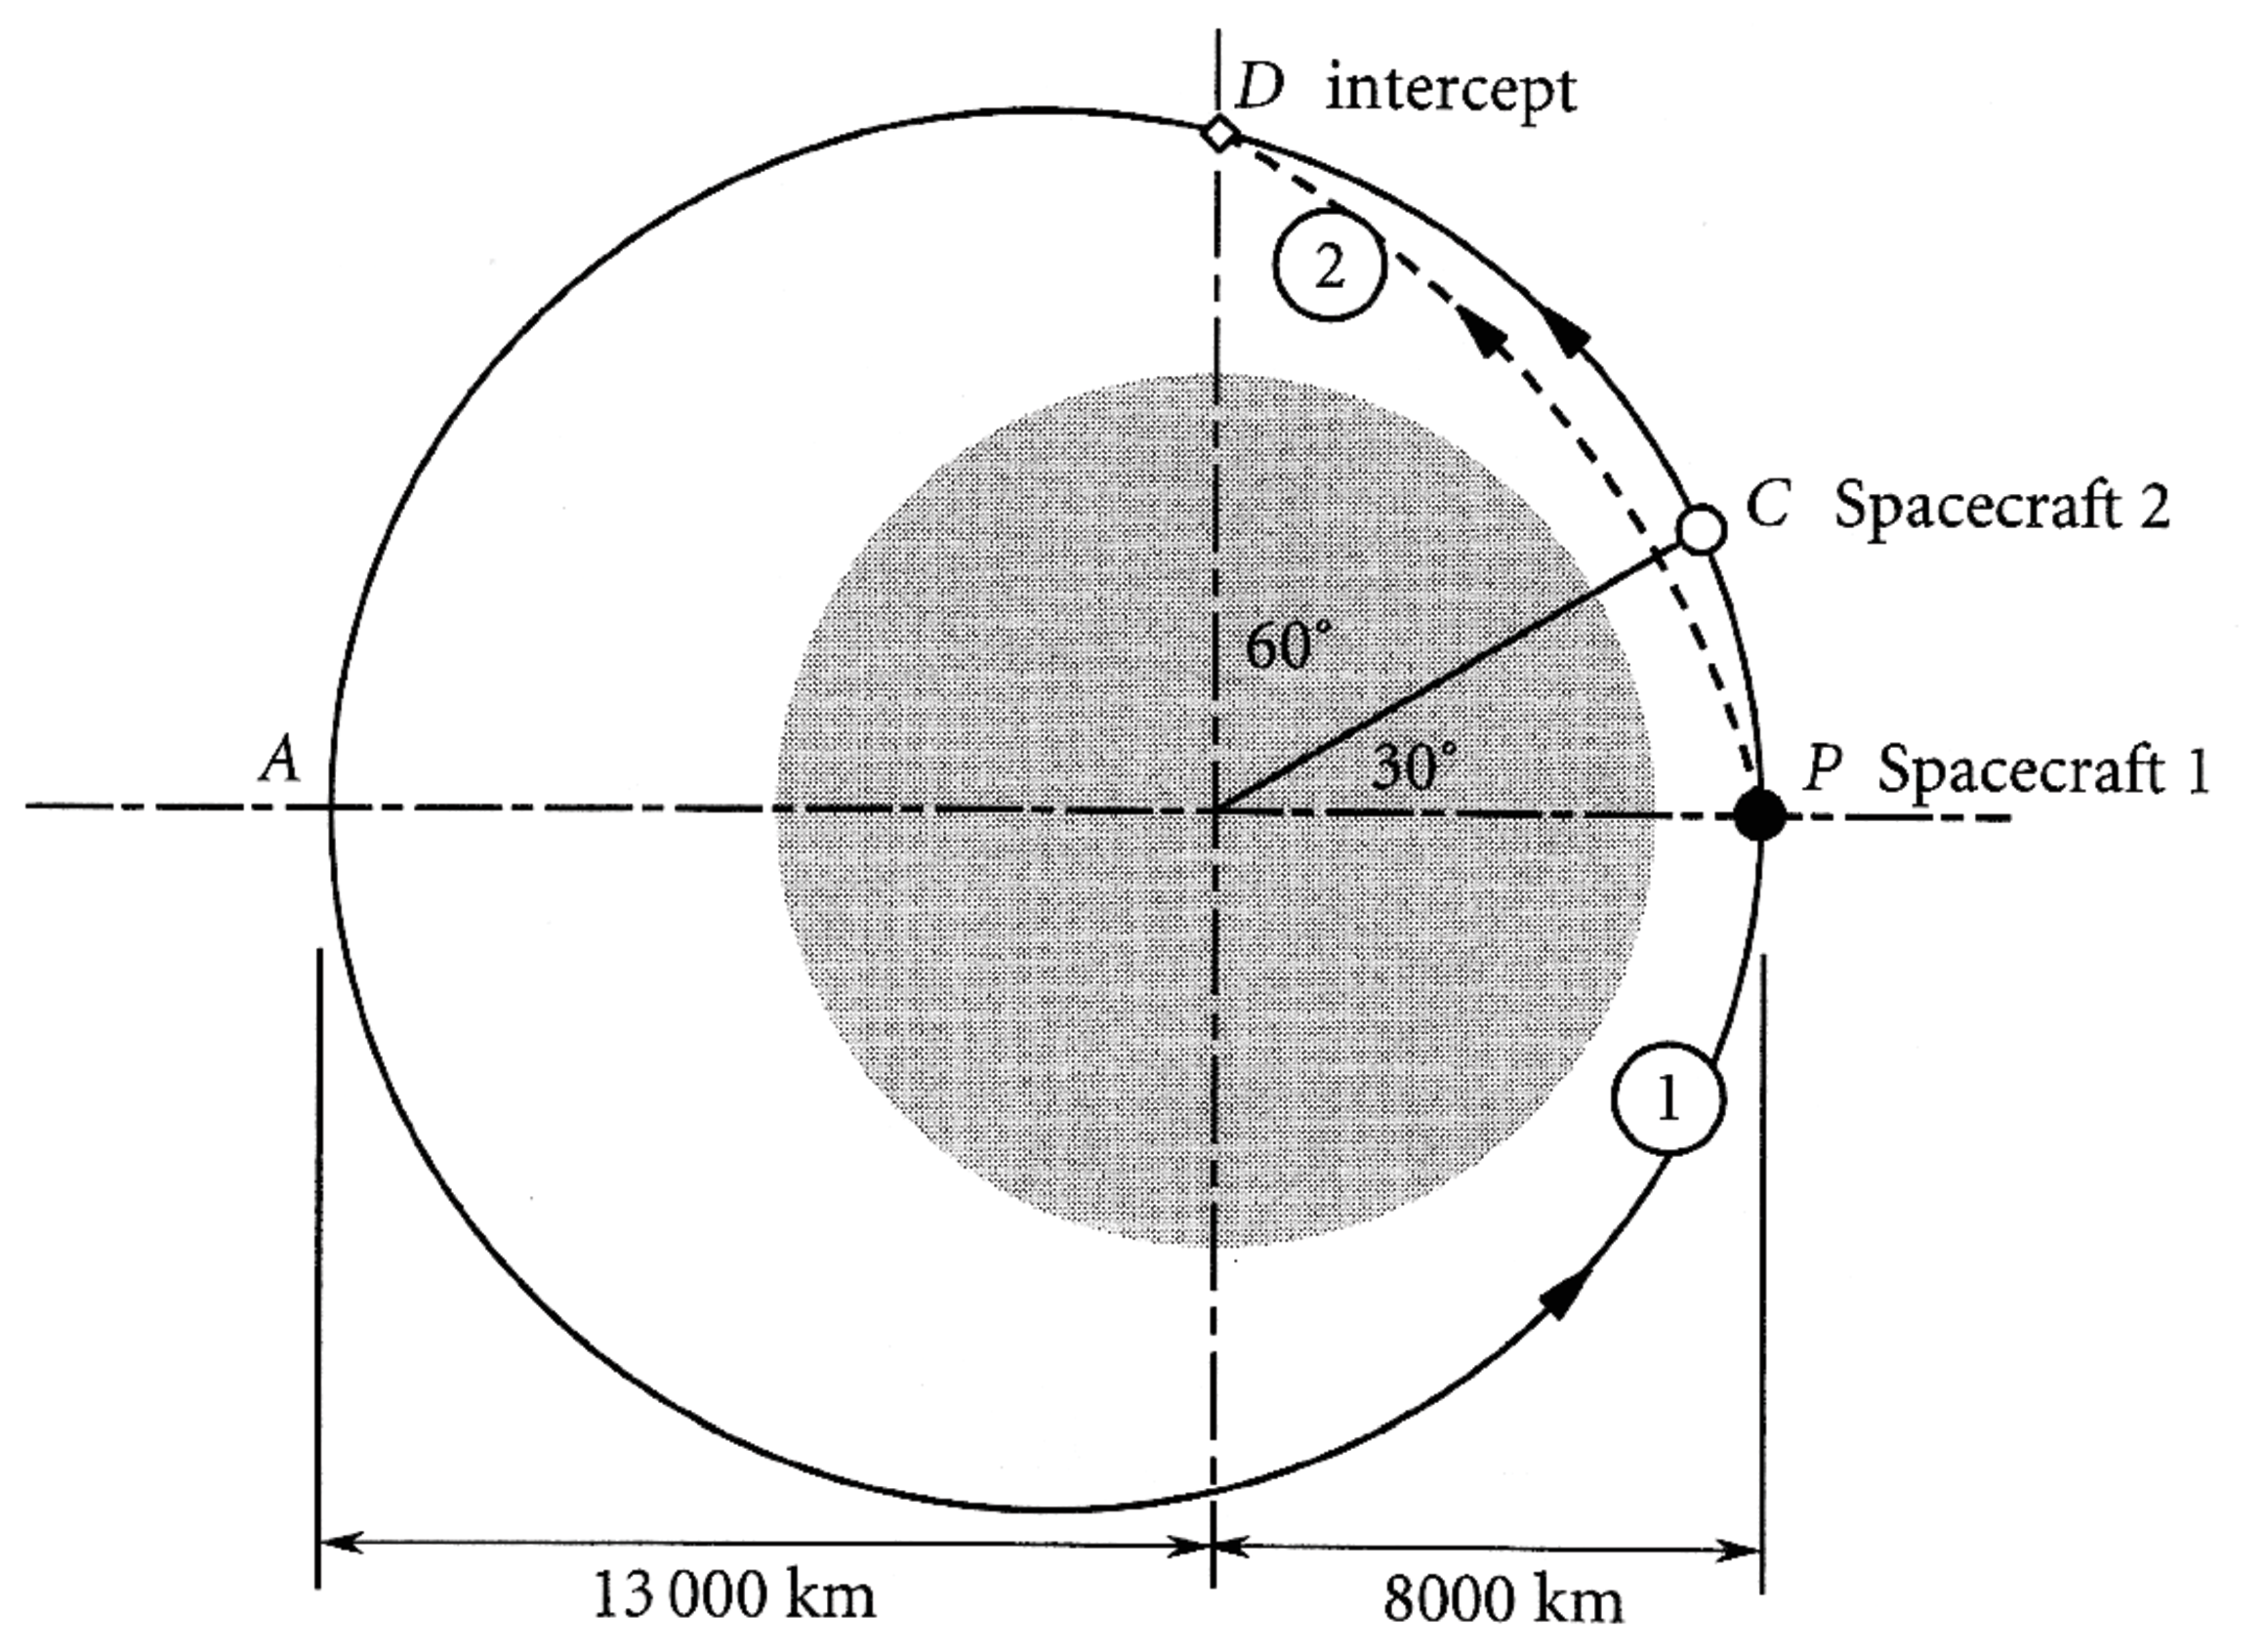
\includegraphics[width=0.45\textwidth]{prob2.eps}}

Recall that the position vector of a mass located at $\theta$ on an orbit with $h,e$ is given by
\begin{align*}
\vec r = r [\cos\theta \hat x + \sin\theta\hat y],\qquad \text{where}\quad r=\frac{h^2}{\mu}\frac{1}{1+e\cos\theta}.
\end{align*}


\begin{subprob}
\item Find the position vector $\vec r_P$ and the velocity vector $\vec v_{P_1}$ of Spacecraft 1 at the point $P$ of Orbit 1.
\item Find the position vector $\vec r_D$ and the velocity vector $\vec v_{D_1}$ of Spacecraft 1 at the point $D$ of Orbit 1.
\item Show that the time required for Spacecraft 2 to move from $C$ to $D$ is $t_{CD}=1.3304\times 10^3$ seconds.
\item The Matlab function \texttt{LambertProb.m} posted at Black Board finds the solution of a Lambert problem. It has the following input and output variables: 

\begin{matlab}
function [vA_vec vB_vec]=LambertProb(rA_vec,rB_vec,tAB,mu)
% Input 1: rA_vec the position vector to the initial point A
% Input 2: rB_vec the position vector to the terminal point B
% Input 3: tAB transfer time from A to B
% Input 4: mu gravitational parameter
% Output 1: vA_vec the velocity vector at A on the transfer orbit
% Output 2: vB_vec the velocity vector at B on the transfer orbit
\end{matlab}
Using this function, find the velocity vector $\vec v_{P_2}$ and $\vec v_{D_2}$ of Spacecraft 1 on the transfer orbit, Orbit 2.

\item Find the required velocity change $\Delta \vec v_P$ and $\Delta \vec v_D$ of Spacecraft 1 at $P$ and $D$
\item Show that the total velocity change is $\Delta v_{total}=6.239\,\mathrm{km/s}$.

\end{subprob}
\end{prob}

%\begin{prob}
%Consider the following two elliptic orbits that have the same eccentricity $e$ and specific angular momentum $h$. The gravitational parameter is given by $\mu$.
%
%\centerline{
%\setlength{\unitlength}{1.8em}\centering\small
%\begin{picture}(20,6)(-10,-3)
%\put(0,0){\vector(1,0){7}}
%\put(0,0){\vector(0,1){3}}
%\put(2,0){\ellipse{7}{4}}
%\put(-2,0){\ellipse{7}{4}}
%\put(0,1.62){\circle*{0.15}}
%\put(0.1,1.9){$A$}
%\put(0,0){\circle*{0.6}}
%\put(-3.2,-2.5){Orbit 1}
%\put(1.6,-2.5){Orbit 2}
%\put(6.5,-0.5){$\hat x$}
%\put(0.2,2.8){$\hat y$}
%\end{picture}}
%
%\begin{subprob}
%\item Assume that $\vec h_1 = \vec h_2 = h \hat z$, i.e. in both orbits, the spacecraft rotates counter-clockwise. Find the magnitude of the required velocity change at $A$ on Orbit 1 to transfer the spacecraft to Orbit 2.
%\item Assume that $\vec h_1 = -\vec h_2 = h \hat z$, i.e. the spacecraft rotates counter-clockwise on Orbit 1, and it rotates clockwise on Orbit 2. Find the magnitude of the required velocity change at $A$ on Orbit 1 to transfer the spacecraft to Orbit 2.
%\end{subprob}
%\end{prob}

\clearpage\newpage

\noindent We wish to design a spacecraft mission to explore the Mars. Suppose that
\begin{gather*}
R_{E}=149.6\times 10^6\,\mathrm{km},\quad
R_{M}=227.9\times 10^6\,\mathrm{km},\\
\mu_E=398600\,\mathrm{km^3/s^2},\quad
\mu_M=42830\,\mathrm{km^3/s^2},\quad
\mu_S=1.3271\times 10^{11}\,\mathrm{km^3/s^2},\\
m_E=5.974\times 10^{24}\,\mathrm{kg},\quad
m_M=6.419\times 10^{23}\,\mathrm{kg},\quad
m_S=1.989\times 10^{30}\,\mathrm{kg}.
\end{gather*}

\begin{prob}
The orbits \circled{1}, \circled{2} of the Earth and the Mars around the Sun, and the Hohmann transfer orbit  \circled{3} from the Earth to the Mars are shown as follows.

\centerline{
\setlength{\unitlength}{1.35em}\centering\footnotesize
\begin{picture}(10,10)(-5,-5)
\put(0,0){\vector(1,0){4.8}}
\put(0,0){\vector(0,1){4.8}}
\put(0,0){\circle{8}}
\put(2.625,0){\circle*{0.15}}
\put(-4,0){\circle*{0.15}}
\put(0,0){\circle*{0.8}}
\put(-4.55,-0.55){$A$}
\put(2.7,-0.55){$D$}
\put(5.0,-0.4){$\hat x$}
\put(0.3,4.5){$\hat y$}
\put(0,0){\circle{5.25}}
\put(-0.656,0){\ellipse{6.625}{6.48}}
\put(1.0,-1.9){\circled{1}}
\put(1.5,-3.0){\circled{3}}
\put(1.9,-4.1){\circled{2}}
\end{picture}}
\vspace*{-0.3cm}
\noindent The location of the Earth at departure, and the location of the Mars at arrival are denoted by the point $D$, and $A$, respectively.

\begin{subprob}
\item Find the velocity $V_{D_1}$ and $V_{D_3}$ with respect to the Sun.
\item Find the velocity $V_{A_3}$ and $V_{A_2}$ with respect to the Sun.
\item Find the travel time $t_{DA}$.
\end{subprob}
\end{prob}


\begin{prob}
In this problem, we determine the possible launch date after December 1, 2016 as follows. On August 27, 2003, the true anomalies of the Mars and the Earth were as follows:
\begin{align*}
\theta_M(0) = 358.13^\circ,\quad \theta_E(0)=230.81^\circ.
\end{align*}
The time duration between those two dates is $4845$ days~\footnote{http://www.timeanddate.com}.

The relative phase between the Mars and the Earth at $t$, namely $\phi(t)=\theta_M(t)-\theta_E(t)$ can be written as
\begin{align*}
\phi(t) = \phi(0) + (n_M - n_E) t,
\end{align*}
where $t$ represents time since August 27, 2003, i.e., $t=0$ on August 27, 2003.

\begin{subprob}
\item Find $\phi(0)$, $n_M-n_E$ in the above equation.
\item Show that the initial phase angle for the Hohmann transfer from the Earth to the Mars is $\phi_0=44.3292^\circ$ from Rendezvous conditions.
\item The launch date can be determined from the following equation:
\begin{align*}
\phi_0 = \phi(0) + (n_M - n_E) t_d + 2\pi k,
\end{align*}
where $k$ is an integer, and $t_d$ denotes the time at which the spacecraft exits the sphere of influence of the Earth, measured from August 27, 2003.  Find the earliest possible time $t_d$ after December 1, 2016, i.e., choose the integer $k$ such that $t_d$ is greater than $4845$ days.

\item The departure date can be found by adding $t_d$ to August 27, 2003. Convert $t_d$ into days, and find the departure date by using the following web site for date calculation: 

\url{http://www.timeanddate.com/date/dateadd.html}.

%What is the corresponding wait time after December 1, 2011 in months (assume that $1\,\mathrm{month}=\frac{365.24}{12}\times 24 \times 3600\,\mathrm{sec}$).
\end{subprob}
\end{prob}


\begin{prob}
In this problem, we design a departure hyperbolic orbit. Suppose that the spacecraft is on a circular orbit around the Earth with an orbital radius of $r=9000\,\mathrm{km}$.
\begin{subprob}
\item Find the radius of the sphere of influence of the Earth, $r_{SOI_E}$. %What is the ratio of $r_{SOI_E}$ to the  orbital radius of the Earth $R_E$.
\item Using your answers to Problem 1, find the hyperbolic excess speed $v_\infty$ required for the Hohmann transfer.
\item Find the specific angular momentum $h$, and the eccentricity $e$ of the departure hyperbolic orbit.
\item Show that the required velocity change $\Delta v$ of the spacecraft at the initial circular parking orbit is $\Delta v = 3.2061\,\mathrm{km/s}$.  

\item Find the location of the rocket firing at the initial circular parking orbit. Answer in terms of the angle measured from the line connecting the Earth and the Sun counterclockwise.
%\item Using the orbital equation $r=\frac{h^2}{\mu}\frac{1}{1+e\cos\theta}$, find the true anomaly $\theta_{SOI}$, when the spacecraft arrives at the surface of the SOI (the answer should be slightly less than $\theta_\infty$).
%\item Find the travel time from the initial circular orbit to the surface of the sphere of influence.
\end{subprob}
\end{prob}

\begin{prob} 
In this problem, we design an arrival hyperbolic orbit. Suppose that the arrival hyperbolic orbit is tangent to the surface of the Mars at the periapsis, i.e. the periapsis radius is equal to the radius of the Mars $r_{M}=3396\,\mathrm{km}$.
\begin{subprob}
\item Find the radius of the sphere of influence of the Mars, $r_{SOI_M}$. %What is the ratio of $r_{SOI_M}$ to the  orbital radius of the Mars $R_M$.
\item Using your answers to Problem 1, find the hyperbolic excess speed $v_\infty$ resulting from the Hohmann transfer.
\item Find the specific angular momentum $h$, and the eccentricity $e$ of the arrival hyperbolic orbit.
\item Show that the velocity of the spacecraft at the surface of the Mars is $v_p=5.6776\,\mathrm{km/s}$. Ignore the atmospheric drag. 
\item Find the location of the arrival point on the surface of the Mars. Answer in terms of the angle measured from the line connecting the Mars and the Sun counterclockwise.
\item Find the aiming radius $\Delta$ of the arrival hyperbolic orbit at the surface of the sphere of influence.
\end{subprob}
\end{prob}


\end{document}

